%%%%%%%%%%%%%%%%%%%%%%%%%%%%%%%%%%%%%%%%%%%%%%%%%%%%%%%%%%%%%%%%%%%%%%
%%%%  SPRIGGAN %%%%%%%%%%%%%%%%%%%%%%%%%%%%%%%%%%%%%%%%%%%%%%%%%%%%%%%
%%%%%%%%%%%%%%%%%%%%%%%%%%%%%%%%%%%%%%%%%%%%%%%%%%%%%%%%%%%%%%%%%%%%%%

\mysubsection{Spriggan Virtues}{advancement-spriggan-virtues}

\myemph{Unless otherwise specified, you can take each Virtue only once.}

\mytable{Y Y Y} {
    \thead{Daredevil (Level 2+)} & \thead{Heroic (Level 4+)} & \thead{Legendary (Level 7+)} \\
} {
    Crown of Elfland\Asterisk & Dreams of Elfland & Bind the Abandoned \\
    Fairy Kiss & The Eye & Extraordinary Medium \\
    Kismet I  & Fealty of the Elements &  Fealty of the Damned\\
    Mortal Charms & Glamour  & Kismet III  \\
    Personality I & Kismet II & Personality III \\
    Reminiscence\Asterisk & Personality II & Saves III  \\
    Saves I & Saves II &  Time Stop \\
    Sight Beyond Sight & Touch of Lethe & - \\
    Strange Medium  & Uncanny Medium & - \\
    Wyrd & - & - 
}






\callout {
    \Asterisk This Virtue can be taken once per \LVL. See details in description.
}


\begin{multicols*}{2}



\myhighlight{Bind the Abandoned}{adv-spriggan-bind-abandoned}

Choose one of the Abandoned whose True Name you know.  They are now bound to you permanently, as if they were a henchman or hireling. They will never be unsummoned or summoned by another, cost no Sovereignty to keep or control, and have unswerving loyalty and treat you as a Small God.  When you reach level 9, you can choose to sacrifice them - through this haruspexy, you can divine the paths that will lead you back to Elfland (this will retire your character).


\myhighlight{Crown of Elfland}{adv-spriggan-rod-elfland}

You gain +1 Sovereignty.  You may choose this Virtue once per Level. 


\myhighlight{Dreams of Elfland}{adv-spriggan-dreams-elfland}

Once per Session, you can cause every Mortal Close to you to fall into a magical slumber for \DUR{d12}.  This works in all ways like the \mypg{Secret: Sleep}{secrets-sleep}. The victims get a \SAVE{Hexes}.  The Dreams of Elfland cannot differentiate between Allies and Monsters.

\myhighlight{Extraordinary Medium}{adv-spriggan-extraordinary-medium}

You obtain a bit of magical material (a dragon's tooth, mithril ore, a ray of sunlight, etc) that could be used in \mypg{Sword Magic}{wonder-sword-magic}.  Tell the Arbiter what this material is.

\myhighlight{The Eye}{adv-spriggan-the-eye}

Your hyper-awareness extends to the metaphysical plane. You can detect Invisible creatures, and immediately see through \mypg{Illusions}{secrets-illusion}. You know if an item is magical by inspecting it for Minutes.

\myhighlight{Fairy Kiss}{adv-spriggan-fairy-kiss}

If you kiss a willing Mortal on the flesh (hand or cheek is fine), they become \effect{Charmed} to you for the rest of the Session. \SAVE{Hexes} negates. You can invoke this Virtue once per Session.

\myhighlight{Fealty of the Damned}{adv-spriggan-damned}

You earn the \mypg{Fealty of the Damned}{forgotten-fealty-damned}, allowing you to summon and control Gremlins, demons, and devils.

\myhighlight{Fealty of the Elements}{adv-spriggan-elements}

You earn the \mypg{Fealty of the Elements}{forgotten-fealty-elements}, allowing you to summon and control Imps and elemental creatures.

\myhighlight{Glamour}{adv-spriggan-fey-glamour}

Once per Session, you may perform the \mypg{Secret of Illusion}{secrets-illusion}. The number of \DICE you may use to invoke the Illusion is equal to half your \LVL, rounded down i.e 2-3rd level 1 die; 4-5 2 dice; etc. There's no need to roll these dice, they're just used to determine the potency of the Illusion. The Illusion lasts for as long as you Concentrate.

\myimage{advancement/Spriggan2}


\myhighlight{Kismet I-III}{adv-spriggan-kismet}

Advance \mybold{all} aspects of your \mybold{Kismet} - \DEATH, \INJURY, and \INSANITY - to the next named level.


\myhighlight{Mortal Charms}{adv-spriggan-mortal-charms}

You can perform the \mypg{Vulgate of Charms}{vulgate-charms} at will.

\myhighlight{Personality I-III}{adv-spriggan-personality}

Advance two \mybold{different} aspects of your \mybold{Personality} \DCUP.


\myhighlight{Reminiscence}{adv-spriggan-reminiscence}

You remember one of the names of \mypg{the Abandoned}{forgotten-abandoned}. You can summon this Abandoned using your Sovereignty. You may choose this Virtue once per Level. 

\myhighlight{Saves I-III}{adv-spriggan-saves}

Advance \mybold{all} Saves to the next named level (Defenseless to Preserved; Preserved to Protected; etc).


\myhighlight{Sight Beyond Sight}{adv-spriggan-sight-beyond-sight}

 You become hyper-aware to the point of prescience.  You cannot be Surprised (including the Drop) and you always win Init (if rolling Init vs a Pooka, you and the Pooka take a turn simultaneously). You can "see" in darkness as if you had \effect{Darksight}.

\end{multicols*}

\begin{center}
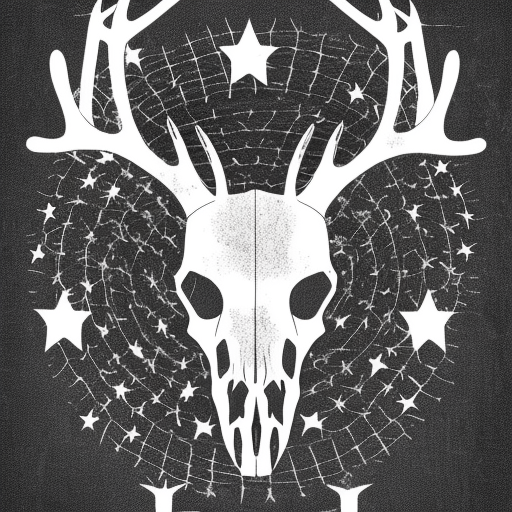
\includegraphics{advancement/Spriggan3}
\end{center}

\begin{multicols*}{2}

\myhighlight{Strange Medium}{adv-spriggan-strange-medium}

You obtain a bit of magical material (a dragon's tooth, mithril ore, a ray of sunlight, etc) that could be used in \mypg{Sword Magic}{wonder-sword-magic}.  Tell the Arbiter what this material is.  You can choose this Virtue once per Rank (once for Daredevil, once for Heroic, and once for Legendary).


\myhighlight{Time Stop}{adv-spriggan-time-stop}

Once per Session, you may stop time for Moments. If invoked during combat, you may take 2 free Maneuver or Combat Actions. A Combat Action does not end your Moment while the Time Stop is in effect.

\cbreak

\myhighlight{Touch of Lethe}{adv-spriggan-touch-lethe}

By touching a Mortal on their exposed skin and whispering in their ear, you can cause them to forget everything that has happened this Session. Any \INSANITY inflicted on the Mortal this Session is likewise forgotten. The Mortal can try a \SAVE{Hexes} to negate the effect - unless they are sleeping, in which case they do not get a Save. You can invoke this Virtue once per Session.

\myhighlight{Uncanny Medium}{adv-spriggan-uncanny-medium}

You obtain a bit of magical material (a dragon's tooth, mithril ore, a ray of sunlight, etc) that could be used in \mypg{Sword Magic}{wonder-sword-magic}.  Tell the Arbiter what this material is.

\myhighlight{Wyrd}{adv-spriggan-wyrd}

You can detect magic, supernatural effects, and general weirdness. 30m range for minor enchantments, charms, and sorceries; 1km range for seriously worrying magical trouble. It might be a premonition, a vision, a cold shudder, a glowing aura, or just a sense that something is "wrong". You can see ghosts and spirits, and they will know and respect you (you never need to roll \INSANITY for seeing shades or horrors). You know if an item is magical by inspecting it for Minutes.


\end{multicols*}
